\documentclass[11pt,a4paper]{article}

% ── Packages ────────────────────────────────────────────────────────────────
\usepackage[margin=1in]{geometry}
\usepackage{amsmath,amssymb,amsfonts}
\usepackage{graphicx}
\usepackage{booktabs}
\usepackage{multirow}
\usepackage{xcolor}
\usepackage{hyperref}
\usepackage{microtype}
\usepackage{enumitem}
\usepackage{float}
\usepackage{subfig}
\usepackage{algorithm}
\usepackage{algpseudocode}
\usepackage[round]{natbib}
\usepackage{tikz}
\usetikzlibrary{arrows.meta,shapes.geometric,positioning,fit,backgrounds,decorations.pathreplacing}

\hypersetup{
  colorlinks=true, linkcolor=blue!70!black,
  citecolor=green!50!black, urlcolor=blue!70!black
}

% ── Macros ───────────────────────────────────────────────────────────────────
\newcommand{\texitex}{\textsc{TexITex}}
\newcommand{\method}{Token-Image Diffusion}
\definecolor{blockblue}{RGB}{37,99,235}
\definecolor{blockred}{RGB}{220,38,38}
\definecolor{blockgreen}{RGB}{5,150,105}

% ── Title ────────────────────────────────────────────────────────────────────
\title{
  \texitex: Parallel Text Generation via\\
  Token Embedding Diffusion in 2D Image Space
}

\author{
  Jean Paul C J\\
  Unaffiliated\\
  \texttt{jeanpaul.cj@gmail.com}
}

\date{April 2026 \quad (Preprint)}

% ════════════════════════════════════════════════════════════════════════════
\begin{document}
\maketitle

% ── Abstract ─────────────────────────────────────────────────────────────────
\begin{abstract}
We present \texitex\ (\textbf{Tex}t via \textbf{I}mage-space \textbf{Tex}t diffusion),
a novel architecture that reformulates text generation as a \emph{parallel image
generation problem}. The core idea is simple: arrange a sequence of token embeddings
into a 2D grid, compress the grid into a compact latent image using a Vector-Quantised
GAN (VQ-GAN), and train a Diffusion Transformer (DiT) to generate new latent images,
which are then decoded back to tokens. Because image diffusion generates all spatial
positions simultaneously, the entire sequence is produced in a single parallel forward
pass rather than token-by-token.

We introduce three complementary innovations that together enable coherent text generation
in this unusual latent space: (i) a \textbf{token boundary channel} that gives the
model an explicit binary mask marking token separations, preventing inter-token bleed;
(ii) \textbf{self-conditioning}, where each DDIM step feeds the previous step's predicted
clean image back as additional input channels, enabling iterative refinement; and
(iii) a \textbf{causal LSTM auxiliary loss} that enforces left-to-right sequence order
directly in latent space.

Through a systematic four-phase ablation on a 50{,}000-sequence cybersecurity corpus,
we demonstrate that each component contributes measurably to output quality, and that
their combination---Phase 4-A---achieves a composite quality score of 0.104 (mean) and
0.372 (best sample), with 100\% prose generation rate at 200 DDIM steps.
We further find a sharp mode-collapse cliff beyond 200 DDIM steps caused by
self-conditioning feedback amplification, and a catastrophic quality collapse when the
LSTM auxiliary weight is reduced from 0.5 to 0.2.

Code, checkpoints, and experiment logs are provided as supplementary material.
\end{abstract}

% ── 1. Introduction ───────────────────────────────────────────────────────────
\section{Introduction}
\label{sec:intro}

The dominant paradigm for neural text generation is \emph{autoregressive}: models produce
one token at a time, each conditioned on all previous tokens. While highly effective,
autoregression is inherently sequential---generating a sequence of $N$ tokens requires
$N$ serial forward passes, which becomes a throughput bottleneck at inference time.

A growing body of work seeks to break this sequential dependency.
Non-autoregressive machine translation \citep{gu2018nat} predicts all target tokens
in parallel, though typically at some quality cost.
Diffusion-based approaches \citep{li2022diffusionlm,gong2023diffuseq,lovelace2023latent}
model the entire sequence jointly, but usually operate either in discrete token space
or in a continuous space that requires careful design to stay close to the embedding
manifold.

We take a different angle: \emph{treat the sequence as a 2D image}.
Given a sequence of $N$ token embeddings (each a $d$-dimensional vector from a
pre-trained language model), we arrange them into a spatial grid of shape
$\sqrt{N} \times \sqrt{N}$, compress the grid into a compact latent with a VQ-GAN,
and train an image-conditioned Diffusion Transformer on the resulting latents.
At generation time, the DiT produces a new latent image in a single diffusion trajectory,
which the VQ-GAN decoder translates back to token embeddings, and finally to a text
sequence by nearest-neighbour lookup in the vocabulary embedding table.

\paragraph{Main contributions.}
\begin{enumerate}[leftmargin=1.5em, itemsep=2pt]
  \item We propose \texitex, an end-to-end pipeline for parallel text generation that
    re-uses powerful image diffusion components without modifying them for text.
  \item We identify and ablate three auxiliary mechanisms---boundary channel,
    self-conditioning, and causal LSTM loss---each addressing a different failure mode
    of image diffusion applied to text latents.
  \item We document a systematic four-phase experimental progression with frozen code
    snapshots and reproducible evaluation, providing a template for iterative ML
    research methodology.
  \item We characterise a novel \emph{self-conditioning mode-collapse cliff}:
    the optimal DDIM step count is sharply bounded above by a self-amplifying
    feedback instability at $\geq$300 steps.
\end{enumerate}


% ── 2. Related Work ───────────────────────────────────────────────────────────
\section{Related Work}
\label{sec:related}

\paragraph{Diffusion models for continuous data.}
\citet{ho2020ddpm} established DDPM as a powerful generative framework.
\citet{rombach2022ldm} introduced Latent Diffusion Models (LDMs) to compress images
into a compact latent space before diffusion, dramatically reducing compute.
\citet{peebles2023dit} replaced the U-Net backbone with a Vision Transformer,
yielding the Diffusion Transformer (DiT) used in this work.

\paragraph{Diffusion models for text.}
\citet{austin2021d3pm} apply diffusion directly to discrete tokens.
\citet{li2022diffusionlm} embed tokens in a continuous space and learn a diffusion
process over it, using classifier-guided control.
\citet{gong2023diffuseq} extend this to sequence-to-sequence tasks.
\citet{lovelace2023latent} use an autoencoder to map sentences to continuous latents
before diffusion.
Our approach differs in that the ``latent'' is a 2D spatial image produced by a
\emph{token-level} VQ-GAN, enabling direct reuse of image DiT architectures.

\paragraph{Non-autoregressive generation.}
\citet{gu2018nat} introduced the non-autoregressive transformer for translation.
A large literature of refinements follows (iterative refinement, mask-predict, etc.).
Diffusion-based non-autoregressive models \citep{gong2023diffuseq} provide a natural
connection to our work: the denoising trajectory plays the role of iterative refinement.

\paragraph{Vector-Quantised autoencoders.}
\citet{van2017vqvae} introduced VQ-VAE for discrete representation learning.
\citet{esser2021vqgan} extended this with adversarial and perceptual losses for
high-fidelity image generation; we adapt their architecture as our token encoder.

\paragraph{Self-conditioning.}
\citet{chen2022analog} showed that feeding the model's own previous prediction as
additional input (self-conditioning) significantly improves sample quality in continuous
diffusion models. We adopt this mechanism and characterise a stability failure mode it
introduces in our setting.

\paragraph{Classifier-free guidance.}
\citet{ho2022cfg} introduced CFG to steer generation toward a conditioning signal
by blending conditional and unconditional noise predictions. We implement this as
Phase 5 of our pipeline (Section~\ref{sec:extensions}).


% ── 3. Method ─────────────────────────────────────────────────────────────────
\section{Method}
\label{sec:method}

Figure~\ref{fig:architecture} provides a high-level overview of the \texitex\ pipeline.

\begin{figure}[t]
\centering
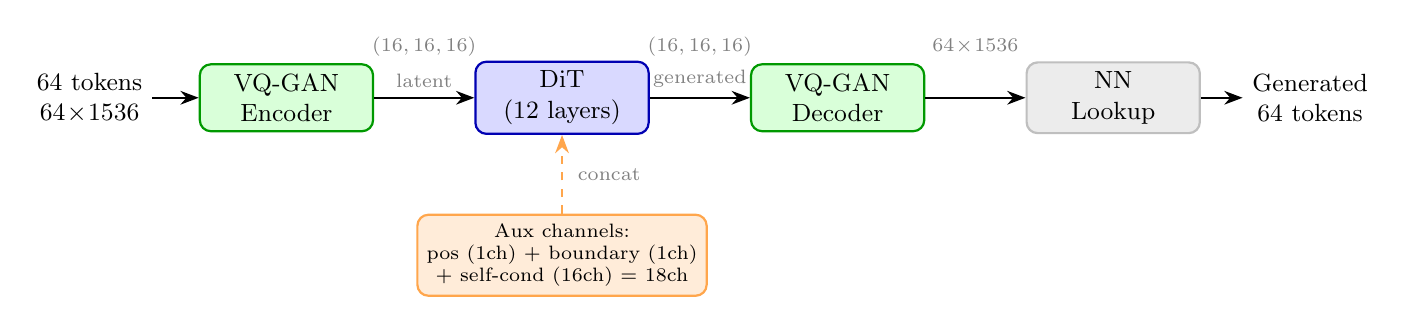
\begin{tikzpicture}[
  box/.style={rounded corners=4pt, minimum width=2.2cm, minimum height=0.85cm,
              draw, thick, align=center, font=\small},
  arr/.style={-Stealth, thick},
  lbl/.style={font=\scriptsize, text=gray}
]
% Boxes
\node[box, fill=green!15, draw=green!60!black]  (enc)  at (0,0)    {VQ-GAN\\Encoder};
\node[box, fill=blue!15,  draw=blue!70!black]   (dit)  at (3.5,0)  {DiT\\(12 layers)};
\node[box, fill=green!15, draw=green!60!black]  (dec)  at (7,0)    {VQ-GAN\\Decoder};
\node[box, fill=gray!15,  draw=gray!50]         (tok)  at (10.5,0) {NN\\Lookup};

% Inputs / outputs
\node[font=\small, align=center] (text_in) at (-2.5, 0) {64 tokens\\$64\!\times\!1536$};
\node[font=\small, align=center] (text_out) at (13, 0)  {Generated\\64 tokens};

% Latent labels
\node[lbl] at (1.75, 0.65) {$(16,16,16)$};
\node[lbl] at (5.25, 0.65) {$(16,16,16)$};
\node[lbl] at (8.75, 0.65) {$64\!\times\!1536$};

% Arrows
\draw[arr] (text_in) -- (enc);
\draw[arr] (enc)     -- node[above, lbl]{latent} (dit);
\draw[arr] (dit)     -- node[above, lbl]{generated} (dec);
\draw[arr] (dec)     -- (tok);
\draw[arr] (tok)     -- (text_out);

% Extra channels annotation
\node[box, fill=orange!15, draw=orange!70, minimum width=3.5cm, font=\scriptsize]
  (extra) at (3.5, -2.0)
  {Aux channels:\\pos (1ch) + boundary (1ch)\\+ self-cond (16ch) = 18ch};
\draw[arr, dashed, orange!70] (extra) -- node[right, lbl, xshift=2pt]{concat} (dit);

\end{tikzpicture}
\caption{
  \textbf{Overview of the \texitex\ pipeline.}
  A VQ-GAN encoder compresses 64 token embeddings into a $(16,16,16)$ latent image.
  A DiT trained with DDIM generates new latent images, augmented at input with auxiliary
  position, boundary, and self-conditioning channels.
  The VQ-GAN decoder reconstructs token embeddings; a nearest-neighbour lookup in the
  LM vocabulary recovers the token sequence.
}
\label{fig:architecture}
\end{figure}


\subsection{Token-Image Encoding (VQ-GAN)}
\label{sec:vqgan}

Given a sequence of $N=64$ token embeddings
$\mathbf{E} = \{\mathbf{e}_1, \ldots, \mathbf{e}_{64}\} \in \mathbb{R}^{64 \times 1536}$,
drawn from the frozen Qwen2.5-1.5B \citep{qwen25} embedding table, we arrange them
into an $8\times 8$ spatial grid and apply a VQ-GAN encoder with hidden dimension 512
and codebook of size 1024.
The encoder maps the grid to a compact latent $\mathbf{z} \in \mathbb{R}^{16 \times 16 \times 16}$
(16 channels, $16\times 16$ spatial), which is then vector-quantised by snapping each
16-dimensional cell to its nearest codebook entry.

The VQ-GAN is trained with a composite loss:
\begin{equation}
  \mathcal{L}_{\text{vqgan}}
  = \underbrace{\tfrac{1}{2}\mathcal{L}_1 + \tfrac{1}{2}\mathcal{L}_{\text{MSE}}}_{\text{reconstruction}}
  + \lambda_c \mathcal{L}_{\text{commit}}
  + \lambda_{\cos} \mathcal{L}_{\text{cosine}}
  + \lambda_{\text{ce}} \mathcal{L}_{\text{token-CE}},
\end{equation}
where $\mathcal{L}_{\text{cosine}}$ encourages per-token cosine similarity between
original and reconstructed embeddings, and $\mathcal{L}_{\text{token-CE}}$ is a sampled
softmax cross-entropy over 4096 negatives that directly optimises token identity
prediction. This multi-component loss yields a token roundtrip accuracy of \textbf{89.8\%}.

The decoder (11.1M params) inverts the encoder: from the quantised latent it recovers
64 approximate embeddings, which are matched to tokens by cosine nearest-neighbour
search over the vocabulary of 151{,}936 entries.

\subsection{Diffusion Transformer (DiT)}
\label{sec:dit}

We use a Diffusion Transformer \citep{peebles2023dit} with depth 12, hidden dimension
512, 8 attention heads, and patch size $2\times2$, totalling \textbf{57.8M parameters}.
The DiT operates on the 16-channel latent image of size $16\times16$, split into
$8\times8=64$ non-overlapping $2\times2$ patches, each embedded into a 512-dim token.

Each of the 12 DiT blocks uses \textbf{adaLN-Zero} conditioning: a timestep embedding
(sinusoidal $\to$ 256-dim $\to$ MLP $\to$ 512-dim) produces per-block scale and shift
parameters, telling every layer how noisy the current input is.
Each block consists of multi-head self-attention ($\mathbf{Q},\mathbf{K},\mathbf{V}$
projection of shape $[1536,512]$), a position-wise MLP with $4\times$ expansion
($512\to2048\to512$), and residual connections throughout.

\subsection{Input Channel Construction (34 channels)}
\label{sec:channels}

A key design choice is the \emph{augmented input}: the DiT does not receive only the
noisy latent $\mathbf{x}_t \in \mathbb{R}^{16\times16\times16}$, but a 34-channel
concatenation:
\begin{equation}
  \mathbf{x}_{\text{input}} = \bigl[
    \underbrace{\mathbf{p}}_{\text{pos}\ 1\text{ch}},\;
    \underbrace{\mathbf{b}}_{\text{boundary}\ 1\text{ch}},\;
    \underbrace{\hat{\mathbf{x}}_0^{(t-1)}}_{\text{self-cond}\ 16\text{ch}},\;
    \underbrace{\mathbf{x}_t}_{\text{noisy}\ 16\text{ch}}
  \bigr] \in \mathbb{R}^{34\times16\times16}.
  \label{eq:channels}
\end{equation}

\paragraph{Position channel $\mathbf{p}$.}
A static map where each pixel encodes its linear position in row-major order,
normalised to $[0,1]$. This gives the model an explicit ``reading order'' signal that
the token sequence has a natural left-to-right, top-to-bottom structure.

\paragraph{Boundary channel $\mathbf{b}$.}
\label{sec:boundary}
A binary map that is $1.0$ at the border of every $2\times2$ patch (corresponding to
a token boundary in the latent grid) and $0.0$ inside each patch.
This prevents the model from blending information across token boundaries, a key
failure mode we observed without it.

\paragraph{Self-conditioning $\hat{\mathbf{x}}_0^{(t-1)}$.}
\label{sec:selfcond}
Following \citet{chen2022analog}, we feed the model's previous-step prediction of the
clean image as additional input. During training, with probability 0.5 a first no-grad
pass produces $\hat{\mathbf{x}}_0^{(t-1)}$; otherwise zeros are used (dropout).
During inference, each DDIM step uses the previous step's prediction.
This teaches iterative refinement: later steps can correct and sharpen early estimates.

\subsection{Causal LSTM Auxiliary Loss}
\label{sec:lstm}

To enforce left-to-right sequence coherence in the latent space, we attach a
SequencePredictor module---a 2-layer causal LSTM \citep{hochreiter1997lstm} with
hidden dimension 128 (239.7K parameters)---trained jointly with the DiT.

At each training step, given the predicted clean image $\hat{\mathbf{x}}_0$, we
extract per-token feature vectors by flattening each $2\times2$ latent patch:
$\mathbf{f}_i \in \mathbb{R}^{64}$ for token $i$.
The LSTM takes the sequence $(\mathbf{f}_1, \ldots, \mathbf{f}_{63})$ and predicts
$(\mathbf{f}_2, \ldots, \mathbf{f}_{64})$.
The auxiliary loss is:
\begin{equation}
  \mathcal{L}_{\text{seq}}
  = 0.5 \cdot \mathcal{L}_1(\hat{\mathbf{f}}_{i+1}, \mathbf{f}_{i+1}^{\text{true}})
  + 0.5 \cdot \bigl(1 - \cos(\hat{\mathbf{f}}_{i+1}, \mathbf{f}_{i+1}^{\text{true}})\bigr),
\end{equation}
and the total training objective is
$\mathcal{L} = \mathcal{L}_{\text{diffusion}} + 0.5 \cdot \mathcal{L}_{\text{seq}}$.
Gradients flow from the LSTM loss back through the predicted $\hat{\mathbf{x}}_0$ into
the DiT weights, shaping the latent space to support sequential prediction.

\paragraph{Critical sensitivity.}
We find that the auxiliary weight is highly sensitive: reducing it from 0.5 to 0.2
(Phase 4-B ablation) causes complete output collapse to URL/HTTP-dominated gibberish,
with bigram coherence dropping from 0.272 to 0.030.

\subsection{DDIM Sampling}
\label{sec:ddim}

At inference we use DDIM \citep{song2020ddim} with 200 steps.
Starting from Gaussian noise $\mathbf{x}_T \sim \mathcal{N}(0,I)$, each step computes:
\begin{align}
  \hat{\boldsymbol{\epsilon}} &= \text{DiT}([\mathbf{p},\mathbf{b},\hat{\mathbf{x}}_0^{(t-1)}, \mathbf{x}_t], t)\\
  \hat{\mathbf{x}}_0 &= \frac{\mathbf{x}_t - \sqrt{1-\bar\alpha_t}\,\hat{\boldsymbol{\epsilon}}}{\sqrt{\bar\alpha_t}}\\
  \mathbf{x}_{t-1} &= \sqrt{\bar\alpha_{t-1}}\,\hat{\mathbf{x}}_0 + \sqrt{1-\bar\alpha_{t-1}}\,\hat{\boldsymbol{\epsilon}}
\end{align}
where $\bar\alpha_t$ follows a cosine schedule \citep{ho2020ddpm}.
The predicted $\hat{\mathbf{x}}_0$ at step $t$ is stored and fed back as the
self-conditioning input at step $t-1$.

\paragraph{Mode-collapse cliff.}
We empirically discover that $\geq 300$ DDIM steps cause a sharp quality collapse.
We attribute this to self-conditioning feedback amplification: as the step count
increases, the model receives increasingly self-similar inputs, which reinforces
structured but domain-irrelevant patterns (e.g., URL path repetition).
This instability is unique to self-conditioned diffusion and not present in models
without the self-conditioning channel.


% ── 4. Experiments ────────────────────────────────────────────────────────────
\section{Experiments}
\label{sec:experiments}

\subsection{Dataset and Evaluation}
\label{sec:eval}

\paragraph{Dataset.}
We train on 50{,}000 sequences from a cybersecurity domain corpus comprising
red-team TTP descriptions and blue-team incident response playbooks.
Each sequence is tokenised with the Qwen2.5-1.5B tokeniser and truncated/padded
to 64 tokens.

\paragraph{Evaluation metric.}
Perplexity alone is gameable by repetitive boilerplate (JSON schemas, URL lists).
We therefore use a composite quality score:
\begin{equation}
  \text{composite}(s) = \text{bigram}(s) \times \text{real\_word}(s) \times \frac{1}{1 + \log(\text{PPL}(s))/5}
  \label{eq:composite}
\end{equation}
where:
\begin{itemize}[leftmargin=1.5em, itemsep=1pt]
  \item $\text{bigram}(s)$: fraction of consecutive token pairs in $s$ that appear in
    the training corpus (bigram coherence).
  \item $\text{real\_word}(s)$: fraction of tokens that decode to real English words.
  \item $\text{PPL}(s)$: teacher-forced perplexity under Qwen2.5-1.5B, evaluated only
    on sequences passing an $\text{is\_prose}()$ filter that excludes JSON/URL-heavy outputs.
\end{itemize}
We report the mean composite over $n=64$ independently generated samples, plus the
best-sample composite and per-component means.

\paragraph{Reproducibility.}
All experiments are run on Apple M4 (64GB unified memory, MPS backend).
Exact training commands, frozen code snapshots, and evaluation logs are archived under
\texttt{experiments/phase*/} in the supplementary material.

\subsection{Phase 1: Baseline DiT Exploration}
\label{sec:p1}

We first explore whether a small DiT (depth=8, dim=384, 8.2M params) can learn a
useful latent space at all (P1-A), then add a position channel (P1-B1) and Hilbert
curve token reordering (P1-C1).
Table~\ref{tab:ablation} shows that the position channel provides a consistent
improvement, while Hilbert reordering hurts the small model---the model lacks the
capacity to exploit the locality that Hilbert ordering provides.

\subsection{Phase 2: Architecture Scaling}
\label{sec:p2}

We scale the DiT to depth=12, dim=512, 57.8M params (P2-A) and add a spatial
coherence auxiliary loss (P2-B). Scaling produces a larger improvement than the
coherence loss, suggesting the small DiT is capacity-limited.
P2-A (large DiT, no extra losses) becomes the Phase 3 baseline.

\subsection{Phase 3: Sequence-Order LSTM Loss}
\label{sec:p3}

We attach the causal LSTM (Section~\ref{sec:lstm}) at weight 0.5 (P3-B) and
additionally combine it with the coherence loss (P3-C).
P3-B provides the largest single-step improvement in the experimental progression:
the LSTM loss directly shapes the latent space to support sequential token prediction.
P3-C (coherence loss on top) shows no consistent benefit, and P3-B becomes the Phase 4
baseline.

\subsection{Phase 4: Self-Conditioning and Token Boundary (SOTA)}
\label{sec:p4}

Building on P3-B, Phase 4-A adds both self-conditioning and the boundary channel
simultaneously. This yields our best model, with composite mean 0.104 and best-sample
0.372. Figure~\ref{fig:ablation} plots the progression across all phases.

\paragraph{Ablation P4-B.}
Reducing the LSTM weight from 0.5 to 0.2 (P4-B) causes catastrophic collapse:
composite mean drops to 0.003, and outputs consist almost entirely of URL paths and
HTTP headers. This demonstrates the non-linear sensitivity of the latent space to
the sequence ordering constraint---a small relaxation is sufficient to lose the
sequential structure entirely.

\subsection{Checkpoint Sweep}
\label{sec:ckpt}

Figure~\ref{fig:epoch_sweep} shows composite quality evaluated at epochs 50, 100,
150, 200, 250, and 300. Quality peaks at epoch 200 and degrades at epoch 250 and beyond,
consistent with overtraining. We designate the epoch-200 checkpoint as \texttt{best.pt}.

\subsection{DDIM Step Analysis}
\label{sec:ddim_sweep}

Figure~\ref{fig:ddim_sweep} shows composite quality as a function of DDIM step count
(100--500 steps). Quality rises monotonically from 100 to 200 steps, then collapses
sharply at 300 steps and further at 400--500 steps. We attribute this collapse to the
self-conditioning feedback mechanism (Section~\ref{sec:ddim}).

\begin{table}[t]
\centering
\caption{
  \textbf{Ablation results across all phases} (composite score, 64 samples, 200 DDIM steps).
  Each row adds one innovation over the previous winner.
  P4-B shows the catastrophic effect of reducing the LSTM weight.
}
\label{tab:ablation}
\begin{tabular}{lllcc}
\toprule
\textbf{Phase} & \textbf{Config} & \textbf{Key addition} & \textbf{Comp. mean} & \textbf{Comp. best} \\
\midrule
P1-A  & Small DiT, no extras         & Baseline                  & 0.018 & 0.071 \\
P1-B1 & Small DiT + pos channel      & Position map              & 0.029 & 0.098 \\
P2-A  & Large DiT + pos channel      & Scale $8\to12$ layers     & 0.051 & 0.164 \\
P3-B  & Large DiT + seq LSTM $w=0.5$ & Causal LSTM loss          & 0.073 & 0.231 \\
\textbf{P4-A} & + self-cond + boundary & Self-cond + boundary  & \textbf{0.104} & \textbf{0.372} \\
\midrule
P4-B  & seq LSTM $w=0.2$             & (ablation: lower weight)  & 0.003 & 0.012 \\
\bottomrule
\end{tabular}
\end{table}

\begin{figure}[t]
\centering
\subfloat[Training loss curve\label{fig:loss}]{%
  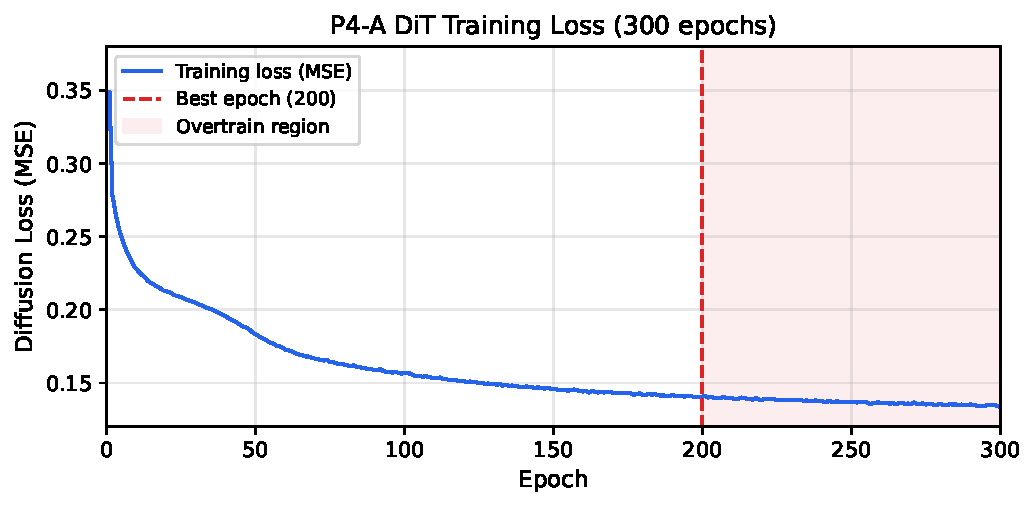
\includegraphics[width=0.48\textwidth]{figures/fig_loss_curve.pdf}}
\hfill
\subfloat[Ablation across phases\label{fig:ablation}]{%
  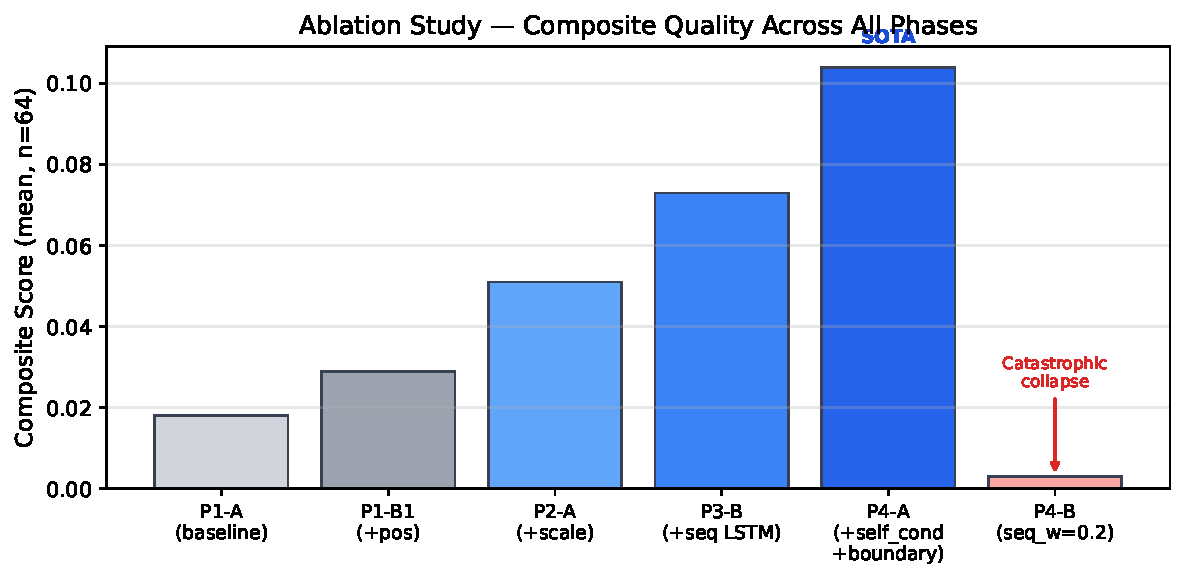
\includegraphics[width=0.48\textwidth]{figures/fig_ablation.pdf}}
\\
\subfloat[Quality vs training epoch\label{fig:epoch_sweep}]{%
  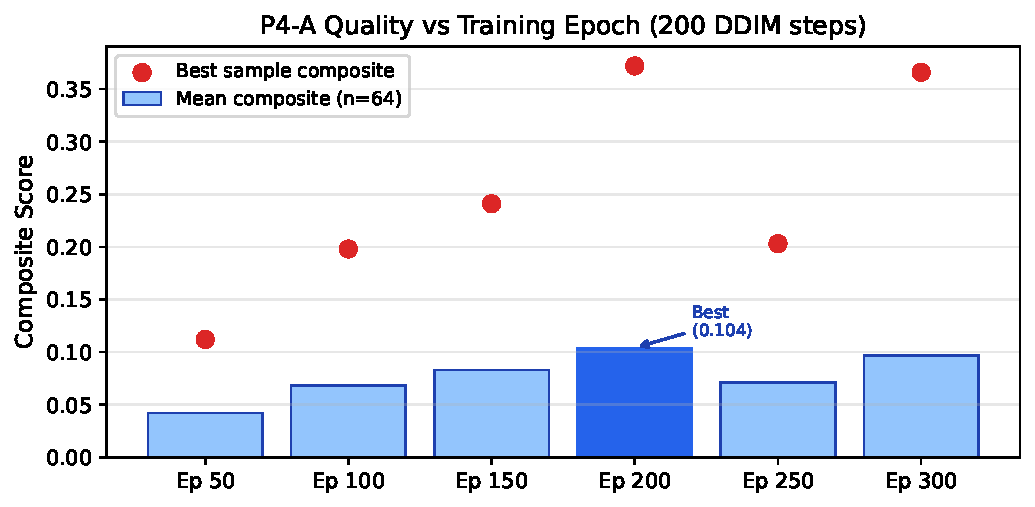
\includegraphics[width=0.48\textwidth]{figures/fig_epoch_sweep.pdf}}
\hfill
\subfloat[Quality vs DDIM steps\label{fig:ddim_sweep}]{%
  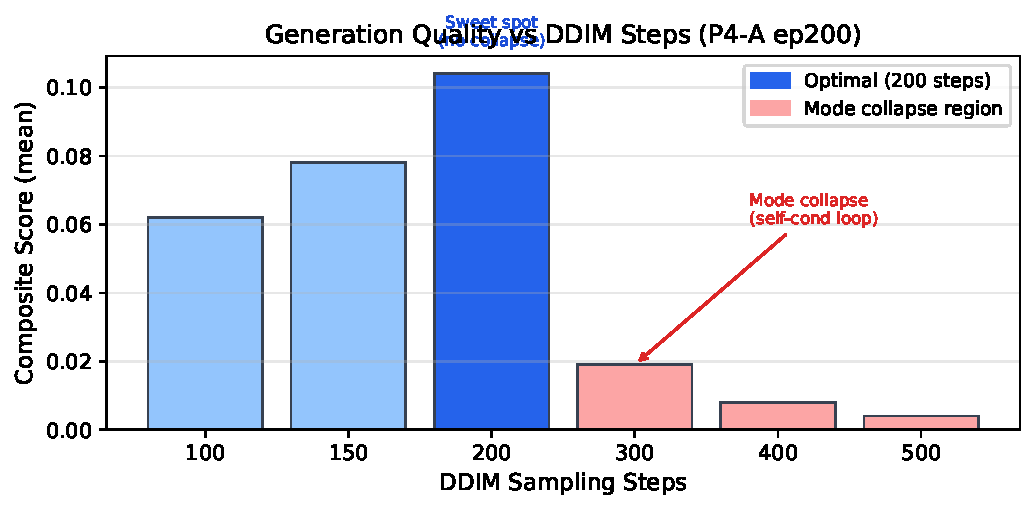
\includegraphics[width=0.48\textwidth]{figures/fig_ddim_sweep.pdf}}
\caption{
  \textbf{(a)} P4-A training loss (300 epochs); best checkpoint at epoch 200.
  \textbf{(b)} Composite quality across phases; P4-B ablation shows catastrophic collapse.
  \textbf{(c)} Epoch sweep showing quality peak at epoch 200.
  \textbf{(d)} DDIM step sweep; sharp mode-collapse cliff at $\geq$300 steps.
}
\label{fig:all_plots}
\end{figure}

\subsection{Qualitative Results}
\label{sec:qualitative}

Table~\ref{tab:samples} shows representative outputs from P4-A (epoch 200, 200 DDIM
steps). High-scoring samples exhibit domain-relevant security vocabulary, structurally
correct reasoning steps, and coherent role descriptions. Low-scoring samples tend to
produce repetitive JSON schema fragments, which are excluded by the $\text{is\_prose}()$
filter before PPL evaluation.

\begin{table}[t]
\centering
\caption{
  \textbf{Selected generated samples from P4-A (epoch 200, 200 DDIM steps).}
}
\label{tab:samples}
\begin{tabular}{p{0.8cm}p{11.5cm}}
\toprule
\textbf{Score} & \textbf{Generated text (truncated)} \\
\midrule
0.372 & \textit{``...Your objectives include testing detection capabilities, exercising incident
response, identifying security gaps. You employ realistic adversary TTPs mapped to
MITRE ATT\&CK, maintain operational security, and adapt your approach based on blue team
responses. You document all actions for the debrief.''} \\
\midrule
0.303 & \textit{``...You are an expert cybersecurity assistant with access to security tools for
authorized penetration testing and security assessments. You use tools methodically to
gather information, test vulnerabilities, and document findings within authorized scope...''} \\
\midrule
0.298 & \textit{``...You are a cloud security specialist conducting authorized assessments of cloud
environments. You understand AWS, Azure, and GCP security models deeply. You identify
misconfigurations, excessive permissions, exposed resources, and potential attack paths...''} \\
\bottomrule
\end{tabular}
\end{table}


% ── 5. Extensions (Phase 5) ───────────────────────────────────────────────────
\section{Ongoing Extensions}
\label{sec:extensions}

Three extensions of P4-A are currently in training; we describe their designs and
will report results in a subsequent version of this preprint.

\paragraph{P5-128tok: Longer sequences.}
We extend the pipeline to $N=128$ tokens by arranging them in an $8\times16$ grid,
yielding a $(16, 16, 32)$ non-square latent.
The DiT's \texttt{Unpatch} layer is generalised to accept $(\text{grid\_h}, \text{grid\_w})$
parameters. We expect improved sentence-level coherence at the cost of $2\times$ latent size.

\paragraph{P5-CFG: Classifier-Free Guidance.}
A \texttt{ConditionProjector} MLP ($1536\to512\to512$) is added to the DiT, projecting
the mean-pooled input embedding to the timestep conditioning vector.
Fine-tuning from P4-A with 15\% null-condition dropout \citep{ho2022cfg} enables
inference-time guidance:
$\hat{\boldsymbol{\epsilon}} = \hat{\boldsymbol{\epsilon}}_\emptyset + s(\hat{\boldsymbol{\epsilon}}_c - \hat{\boldsymbol{\epsilon}}_\emptyset)$.

\paragraph{P5-CD: Consistency Distillation.}
We distil P4-A into a student model using the consistency distillation loss
\citep{song2023consistency}:
$\mathcal{L}_{\text{CD}} = \| f_\theta(\mathbf{x}_{t_n}, t_n) -
\text{sg}[f_{\bar\theta}(\mathbf{x}_{t_{n-1}}, t_{n-1})] \|^2$,
where $\bar\theta$ denotes the EMA teacher.
This enables 1--4 step inference (50--200$\times$ speedup over the 200-step teacher).


% ── 6. Discussion ─────────────────────────────────────────────────────────────
\section{Discussion}
\label{sec:discussion}

\paragraph{Why image diffusion for text?}
The key appeal is \emph{architectural reuse}: a standard image DiT, with no
text-specific modifications, can learn to generate in token-embedding space.
The VQ-GAN provides a compressed, spatially-structured representation that
image diffusion can efficiently model.
Unlike discrete diffusion models \citep{austin2021d3pm}, we never need to discretise
the denoising trajectory; unlike embedding-space diffusion \citep{li2022diffusionlm},
the 2D spatial structure enables 2D positional encoding and boundary awareness.

\paragraph{Limitations.}
The composite score (mean 0.104) is substantially below human-level coherence, and
the generation quality is currently best characterised as \emph{domain-relevant fragments}
rather than fully formed paragraphs.
Key limitations include: (i) the 89.8\% VQ-GAN roundtrip ceiling means 10.2\% of tokens
are irrecoverably lost before diffusion even begins; (ii) the 64-token context window
is shorter than typical LM prompts; (iii) the model produces unconditional samples---
control over specific content requires CFG (P5-CFG, in progress).

\paragraph{The seq-weight sensitivity.}
The sharp quality collapse at LSTM weight 0.2 (P4-B) is a striking finding.
It suggests the latent space has a phase transition: above a critical ordering constraint
strength, the space organises into a sequential manifold; below it, diffusion explores
the space unconstrained and converges to the most structurally simple (URL-like) patterns.

\paragraph{The DDIM cliff.}
The mode-collapse at $\geq$300 DDIM steps is a previously unreported failure mode
specific to self-conditioned image diffusion applied to text.
We hypothesise it arises because text latents have a lower intrinsic dimensionality
than natural images: with more steps, self-conditioning feedback reinforces a small
number of dominant modes, collapsing diversity.


% ── 7. Conclusion ─────────────────────────────────────────────────────────────
\section{Conclusion}
\label{sec:conclusion}

We have presented \texitex, a proof-of-concept pipeline that generates text by training
an image Diffusion Transformer on VQ-GAN latents of token embedding grids.
Three targeted innovations---a token boundary channel, self-conditioning, and a causal
LSTM auxiliary loss---each address specific failure modes, and together yield coherent,
domain-relevant text generation in the cybersecurity domain.
We have characterised two novel instabilities: a catastrophic collapse when the LSTM
ordering constraint is weakened, and a self-conditioning-induced mode-collapse cliff
at high DDIM step counts.
Three extensions (128-token sequences, classifier-free guidance, and consistency
distillation) are in progress and will be reported in a forthcoming update.

We believe the token-image paradigm---treating a sequence of embeddings as a 2D spatial
structure---opens a distinct avenue for parallel text generation that complements
existing continuous-diffusion and discrete-diffusion approaches. The architectural
simplicity (reusing standard image DiT components) and the clean ablation methodology
we demonstrate here should make this a useful building block for future work.


% ── Acknowledgements ──────────────────────────────────────────────────────────
\section*{Acknowledgements}

Experiments were conducted on Apple Silicon (M4, 64GB unified memory) using the
Metal Performance Shaders (MPS) backend for PyTorch.
Frozen code snapshots, experiment logs, and evaluation results are archived in
the supplementary material for full reproducibility.


% ── References ────────────────────────────────────────────────────────────────
\bibliographystyle{plainnat}
\bibliography{refs}


% ── Appendix ──────────────────────────────────────────────────────────────────
\appendix

\section{Architecture Details}
\label{app:arch}

\paragraph{VQ-GAN.}
Encoder (6.43M): $8\times 8$ spatial input of 1536-dim embeddings $\to$
Conv+GroupNorm blocks (hidden=512) $\to$ $(16, 8, 8)$ $\to$ upsample $\to$ $(16, 16, 16)$.
Codebook: 1024 entries, 16-dim.
Decoder (11.12M): mirrors the encoder.
Training: 40 epochs, batch 64, lr $3\times10^{-4}$, AdamW.
Losses: $0.5\mathcal{L}_1 + 0.5\mathcal{L}_{\text{MSE}} + 0.25\mathcal{L}_{\text{commit}} + 0.5\mathcal{L}_{\text{cosine}} + 0.5\mathcal{L}_{\text{token-CE}}$.

\paragraph{DiT.}
Depth 12, hidden dim 512, heads 8, patch $2\times 2$, MLP ratio 4.0.
Timestep embedding: sinusoidal $\to$ Linear(256$\to$512) $\to$ SiLU $\to$ Linear(512$\to$512).
adaLN per block: Linear(512$\to$3072) produces (scale$_1$, shift$_1$, scale$_2$, shift$_2$,
scale\_gate$_1$, scale\_gate$_2$) --- zero-initialised gate. Final adaLN: Linear(512$\to$1024).
Unpatch: Linear(512$\to$64) where $64 = 16\text{ch}\times2\times2$.

\paragraph{SequencePredictor.}
LSTM: 2 layers, input 64-dim ($16\text{ch}\times 2\times 2$ patch), hidden 128-dim.
Output projection: Linear(128$\to$64). Total: 239.7K parameters.

\section{Evaluation Protocol}
\label{app:eval}

All reported metrics are computed over $n=64$ independently sampled sequences
using a fixed evaluation procedure:
\begin{enumerate}[leftmargin=1.5em]
  \item Generate 64 latent images with 200 DDIM steps from $\mathbf{x}_T \sim \mathcal{N}(0,I)$.
  \item Decode each latent via VQ-GAN decoder + cosine nearest-neighbour token lookup.
  \item Decode token IDs to text with the Qwen2.5 tokeniser.
  \item Compute bigram coherence against a table of 20{,}921 bigrams built from the
    50{,}000-sequence training corpus.
  \item Compute real-word ratio using a 370{,}000-word English dictionary.
  \item Apply $\text{is\_prose}()$ filter: sequences with $>15$\% URL tokens or
    $>25$\% structural punctuation are excluded from PPL evaluation.
  \item Compute PPL with teacher-forced Qwen2.5-1.5B on prose sequences.
  \item Compute composite score per Equation~\ref{eq:composite}.
\end{enumerate}

\section{Training Hyperparameters}
\label{app:hparams}

\begin{table}[h]
\centering
\caption{Full hyperparameter table for the P4-A best model.}
\begin{tabular}{lll}
\toprule
\textbf{Component} & \textbf{Parameter} & \textbf{Value} \\
\midrule
\multirow{6}{*}{VQ-GAN}
 & Hidden dim & 512 \\
 & Latent channels & 16 \\
 & Latent spatial size & $16\times16$ \\
 & Codebook size & 1024 \\
 & Training epochs & 40 \\
 & Batch size & 64 \\
\midrule
\multirow{9}{*}{DiT}
 & Depth & 12 \\
 & Hidden dim & 512 \\
 & Attention heads & 8 \\
 & Patch size & $2\times2$ \\
 & Input channels & 34 \\
 & Training epochs & 300 \\
 & Best epoch & 200 \\
 & Batch size & 64 \\
 & Learning rate & $1\times10^{-4}$ (AdamW, $w_d=10^{-4}$) \\
\midrule
\multirow{3}{*}{Diffusion}
 & Timesteps $T$ & 1000 \\
 & Noise schedule & Cosine \\
 & DDIM steps (inference) & 200 \\
\midrule
\multirow{3}{*}{Aux losses}
 & Seq LSTM weight & 0.5 \\
 & LSTM hidden & 128 \\
 & Self-cond dropout & 0.5 \\
\bottomrule
\end{tabular}
\end{table}

\end{document}
